%    Documentation for Irrigation Control Project
%    Copyright (C) 2017  Gregory Raven
%
%    This program is free software: you can redistribute it and/or modify
%    it under the terms of the GNU General Public License as published by
%    the Free Software Foundation, either version 3 of the License, or
%    (at your option) any later version.
%
%    This program is distributed in the hope that it will be useful,
%    but WITHOUT ANY WARRANTY; without even the implied warranty of
%    MERCHANTABILITY or FITNESS FOR A PARTICULAR PURPOSE.  See the
%    GNU General Public License for more details.
%
%    You should have received a copy of the GNU General Public License
%    along with this program.  If not, see <http://www.gnu.org/licenses/>.

\chapter{An HTML5 Controller}

The controller GUI is an HTML5 web page.  The project was developed with the 
Chromium browser in Ubuntu 16.04.

There was no attempt to fix problems with cross-browser compatibility issues.  
Plain HTML5 and CSS was used throughout.  The HTML was manipulated directly via 
the ``Document Object Model'' (DOM) technology in the web browser.  This is a 
bare-bones interface with no fancy features.

\begin{figure}[h]
	\centering
    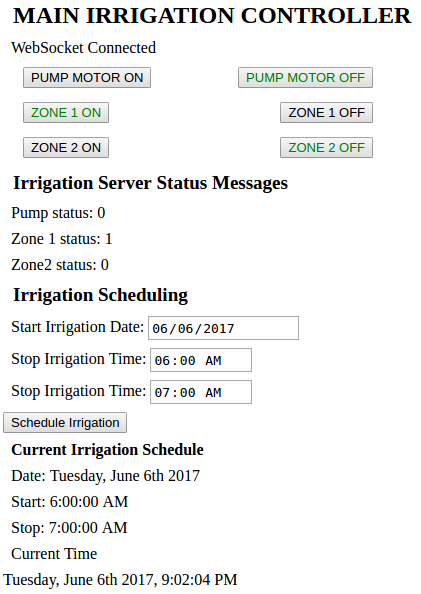
\includegraphics[width=0.5\textwidth]{photos/browser_full.png}
	\centering\bfseries
	\caption{The Irrigation Controller as seen with a Chromium Browser}
\end{figure}

Manual control buttons for the zone solenoids and the pump motor are at the 
top.  The user can enter a schedule date and start and stop times.  Clicking 
the ``Schedule'' button sends the requested irrigation schedule to the server.  
The server responds with a message which updates the displayed schedule.  No 
rigorous checking of inputs is done.

The current date and time are shown in the last line of the controller page.
Originally, the time and date were obtained from the host computer.  This
information is redundant, as the user will have access to the host system time
via some other GUI.  Also, the irrigation timing events will be use the system
time on the BBGW server.  It makes sense to show display the BBGW system time, as
there could be a discrepancy if the BBGW uses a real time clock which has significant
error.

The HTML has been modified to show the BBGW server's system time sent via WebSocket.
The time is updated every minute.  This should be sufficient precision for this
particular application.
